%!TEX root = ../main.tex
\chapter{Influence of the number of triggered channels and parametrization in simulation.}
\label{appendix:ped_shift}

The correction applied function of the number of hits above 0.5 MIPs in a chip is only a global correction shifting the mean of the time distribution. However, it does not correct for the increase of the width of the time distribution. The increase of the width can be clearly seen in figure \ref{fig:ped_shift_dist_para}. This increase has to be implemented in the simulation in order to match the timing distribution of electrons without also influencing the time distribution for muons. A parametrization extracted from data is therefore implemented in the simulation. This parametrization assumes the following, the effect is additional to the seen muon resolution giving then:
\begin{equation*}
	\text{RMS}_{\text{obs}}^2 = \text{RMS}_{\mu}^2 + \text{RMS}_{\text{effect}}^2
\end{equation*}
The $\text{RMS}_{\text{effect}}$ is extracted from data by fitting with a function of the following form:
\begin{equation*}
	f(t) = A \times e^{-\frac{(t-\mu_1)^2}{2(\sigma_1^2 + \sigma_{effect}^2)}} + B* \times e^{-\frac{(t-\mu_2)^2}{2(\sigma_2^2 + \sigma_{effect}^2)}} + C
\end{equation*}

\begin{figure}[htbp!]
	\begin{subfigure}[t]{0.49\textwidth}
		\centering
		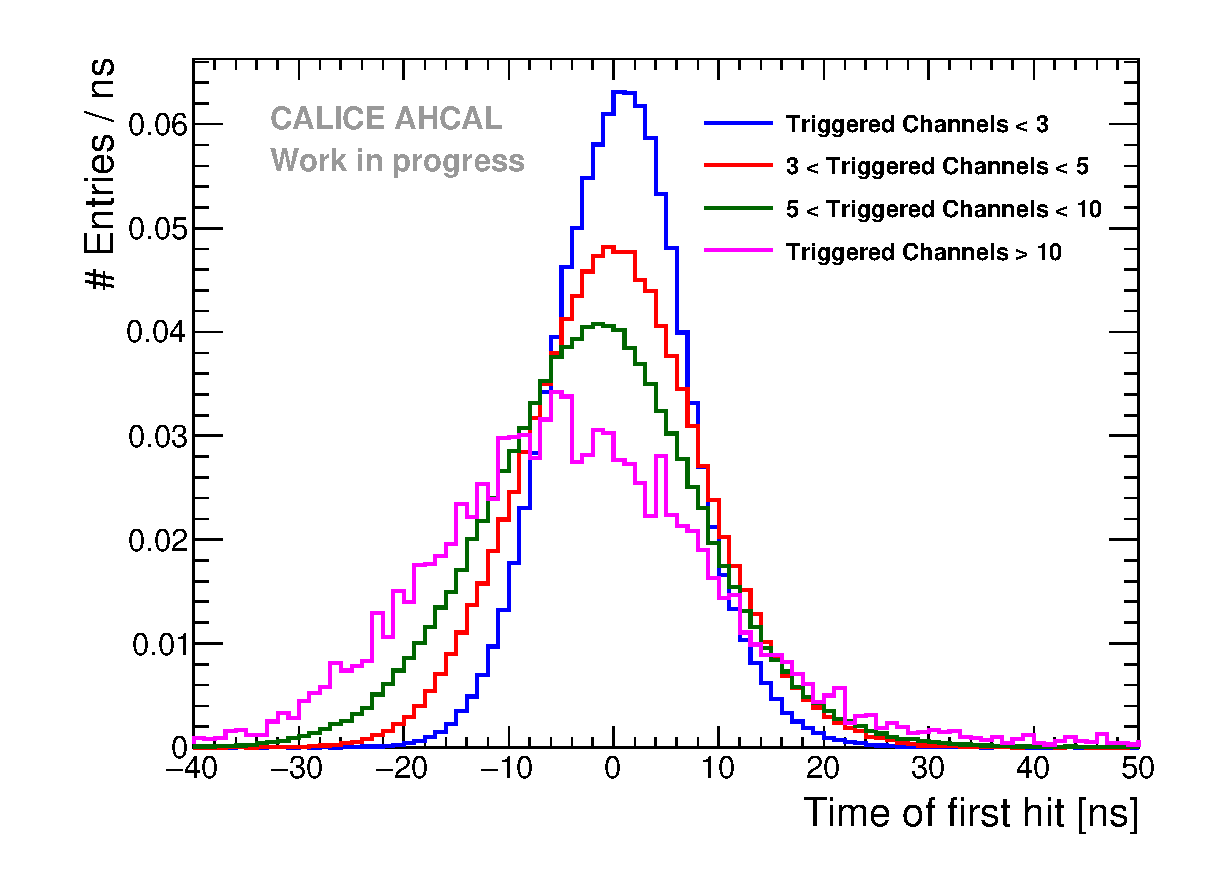
\includegraphics[width=1\linewidth]{../Thesis_Plots/Timing/Electrons/Plots/TimingHitsBins_20GeV.eps}
		\caption{} \label{fig:ped_shift_dist_para}
	\end{subfigure}
	\hfill
	\begin{subfigure}[t]{0.49\textwidth}
		\centering
		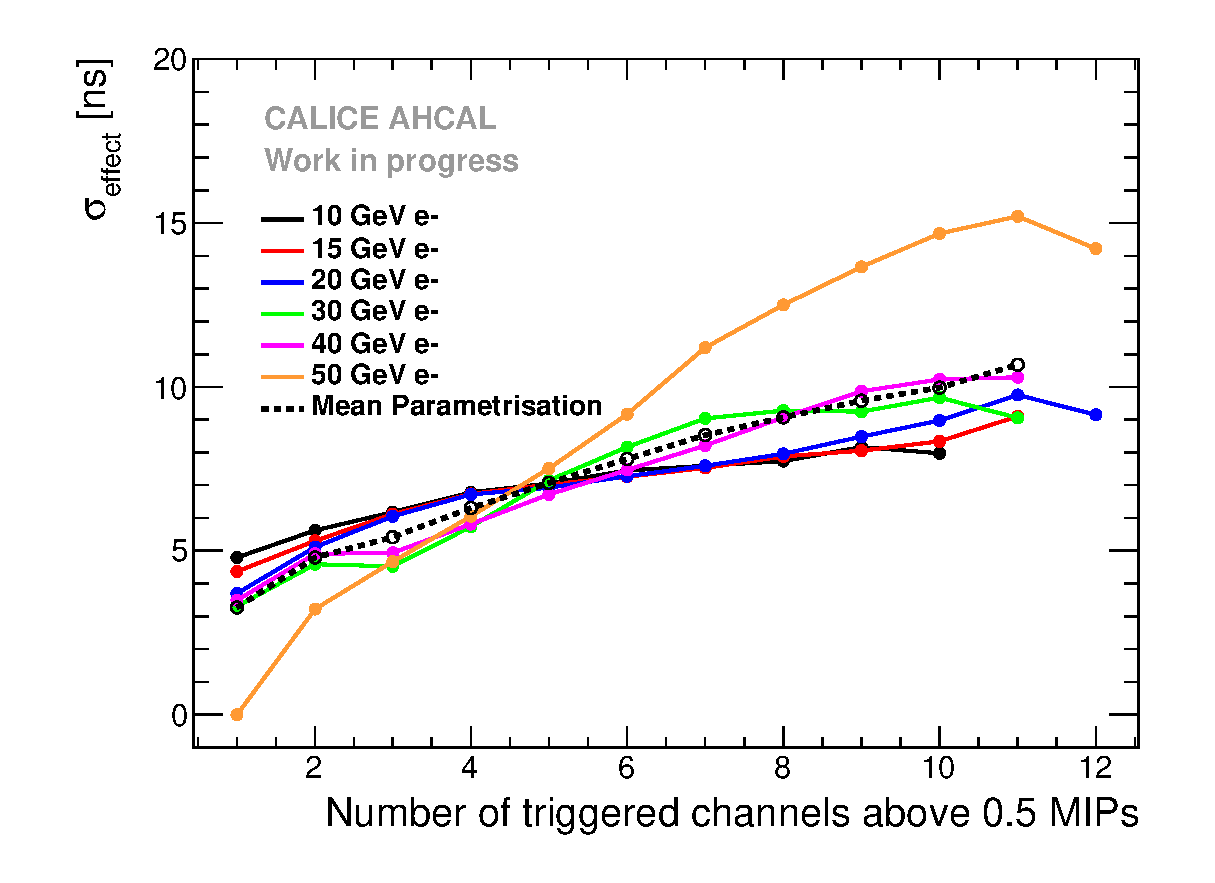
\includegraphics[width=1\linewidth]{../Thesis_Plots/Timing/Electrons/Plots/MeanParametrisation.eps}
		\caption{} \label{fig:para_fit}
	\end{subfigure}
	\caption{\subref{fig:ped_shift_dist_para}) Time of the first hit distribution for different binning of number of triggered channels in a chip. The distribution width is increasing with the number of triggered channels in a chip due to the remaining of the observed effect. \subref{fig:para_fit}) $\sigma_{effect}$ extracted function of the number of triggered channels in a chip for each energies. $\sigma_{effect}$ increases up to 12-15 ns with the number of triggered channels in a chip.}
\end{figure}

The parameters $\mu_1$, $\sigma_1$, $\mu_2$ and $\sigma_2$ are fixed from table \ref{table:time_res_sim}. By plotting $\sigma_{effect}$ extracted as a function of the number of triggered channels in a chip, one can extract a parametrization. This is done for each electron energy point as shown in figure \ref{fig:para_fit}. One can observe that each parametrization curve is slightly different for each energy. This may be due to the fact that each energy affects not exactly the same part of the detector. Moreover, the 50 GeV parametrization looks very different than the others. All time distributions for all chips and layers have been investigated manually in order to understand the different but no clear reason has been found.

To accommodate this, a mean parametrization is used in simulation with an envelope used as uncertainty as shown in figure \ref{fig:mean_para}. Only points up to 10-11 number of channels are extracted from data. Above this, the value of $\sigma_{effect}$ is extrapolated. This should in principle have relatively a small effect for electrons as mainly 6-10 hits are expected per chip. However, the effect may be relevant for pions.

\begin{figure}[htbp!]
	\centering
	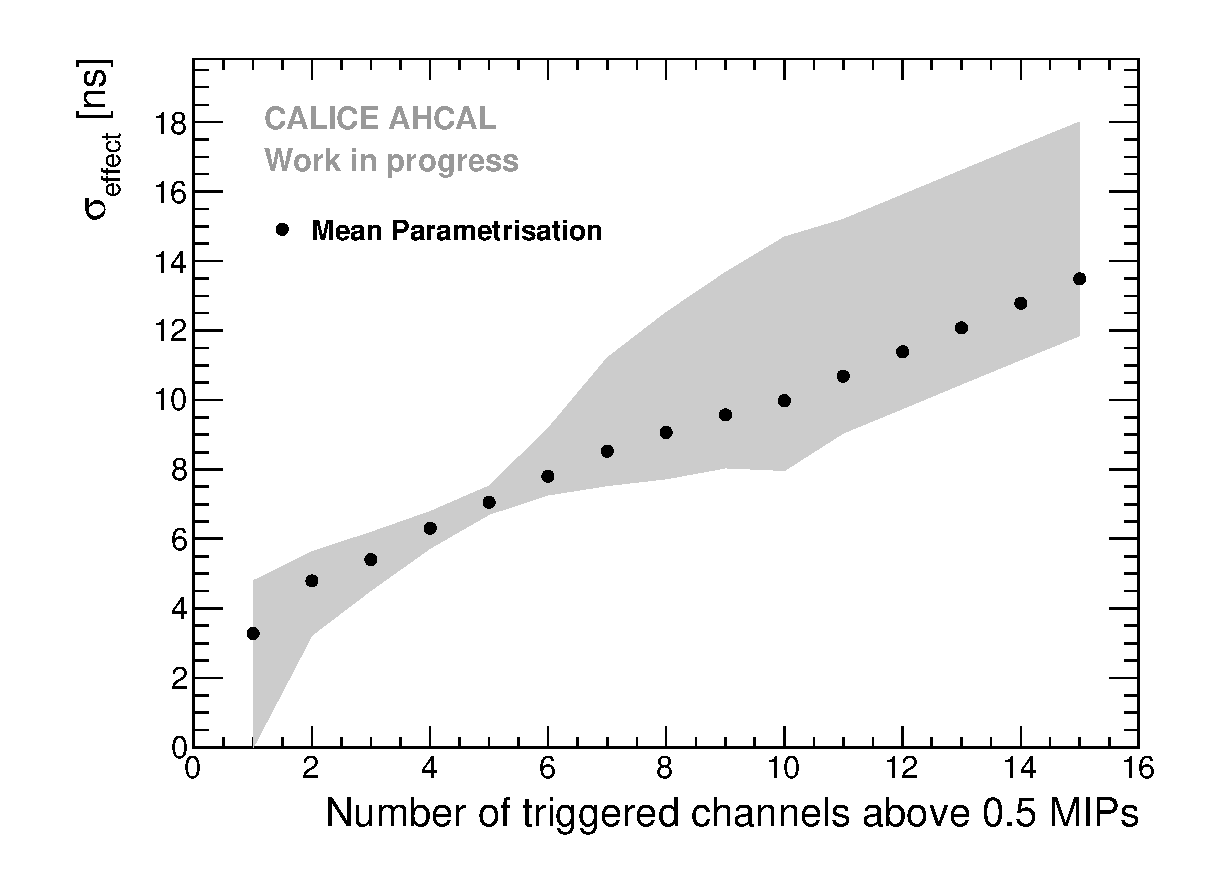
\includegraphics[width=0.7\linewidth]{../Thesis_Plots/Timing/Electrons/Plots/MeanParametrisationWithSystErrors.eps}
	\caption{Mean parametrization of $\sigma_{effect}$ as a function of number of triggered channels. The grey area represents the uncertainty on the parametrization.}
	\label{fig:mean_para}
\end{figure}
